%Todos los capitulos se pueden compilar por separado, hace más fácil el trabajo
%de escritura.
\documentclass[11pt, twoside]{book}
\usepackage[utf8]{inputenc}
\usepackage[OT1]{fontenc}
\usepackage{imunam-tesis}
\usepackage[subpreambles=false]{standalone}
\usepackage[spanish, mexico]{babel}
\usepackage{mathpazo} %Fuente principal
\usepackage{eulervm} %Fuente en el entorno matemático
\usepackage{mathtools} % Para las flechas de inclusión 

\usepackage{float}

% commando necesario para generar los índices
\makeindex

% Paquete para hace gráficas
\usepackage{pgfplots}
\pgfplotsset{compat=1.11} 

% Paquete para incluir dos subfiguras en una misma figura
\usepackage{subcaption}

% Configura tikz para los diagramas
\usepackage{tikz}
\usetikzlibrary{cd}
\usetikzlibrary{arrows}
\usetikzlibrary{decorations.markings}
\tikzset{
commutative diagrams/.cd,
arrow style=tikz,
diagrams={>=stealth}}

% Compila la bibliografia con biblatex
\usepackage[
  style=ieee,
  backend=biber,
  sorting=ynt
]{biblatex}

\addbibresource{bibliografia.bib}

\graphicspath{{imagenes/}{../imagenes/}}

% Usa romanos en las listas enumeradas
\renewcommand{\labelenumi}{\roman{enumi}}

\usepackage{mathtools}

\begin{document}
\chapter{Preliminares}
Esta plantilla permite la escritura de una tesis completa incluyendo además
comandos adicionales que hace más fácil el trabajo de escritura

El archivo \textit{premable.tex} contiene los comandos especiales de acuerdo a
los requerimientos de cada documento, puede ser modificado libremente. Es
importante si se van a usar paquetes adicionales agregarlos ahí para poder
compilar correctamente cada capítulo por separado.

\section{Imágenes} \label{sec:imagenes}
Todas las imágenes se deben guardar en la carpeta \textit{imagenes}. Luego
pueden ser incluidas en el documento con el comando usual:

\begin{figure}[ht]
  \centering
  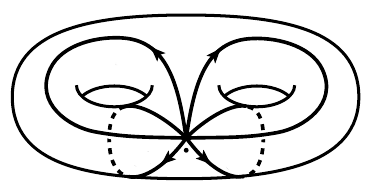
\includegraphics{bitorus.png}
  \caption{Ejemplo de figura. Un toro doble}
  \label{fig:dobletoro}
\end{figure}

Como siempre una imagen puede ser referida posteriormente, como la figura
\ref{fig:dobletoro} que insertamos hace rato.

Otro comando importante es \verb|\imagenpendiente| que como su nombre lo
indica permite añadir un cuadro en el lugar donde posteriormente pondremos una
imagen que tal vez aún no tenemos lista. Se puede agregar además un mensaje que
nos recuerde qué pondremos ahí.

\begin{figure}[ht]
  \centering
  \figurapendiente{aqui pondré un bonito diagrama luego}
  \caption{Ejemplo de figura pendiente}
  \label{fig:pendiente1}
\end{figure}


Finalmente, y aunque esto no es exclusivo de esta plantilla, las figuras
generadas con \textit{Tikz} se pueden importar con el mismo comando que
cualquier otra imagen.

\begin{figure}[ht]
  \centering
  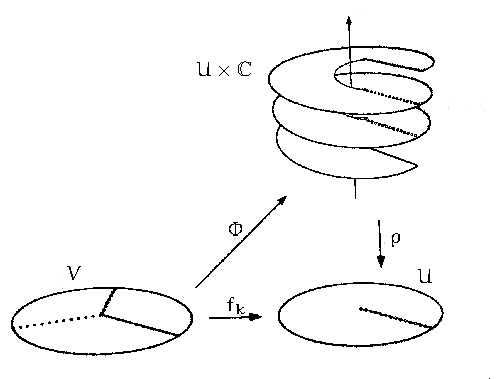
\includegraphics{branchedcover.tex}
  \caption{Ejemplo de figura generada con Tikz}
  \label{fig:tikz1}
\end{figure}


\section{Definiciones, teoremas, corolarios, lemas y pruebas}

El único propósito de esta sección es mostrar cómo funcionan los estilos para
definiciones, teoremas, corolarios y pruebas

\begin{teorema}[Seifert-Van Kampen] %
  Los grupos dados por las imágenes \(\ j_{1*}(G_1)\) y 
  \(j_{2*}(G_2)\) generan a \(G\). Más aún, para cualquier grupo arbitrario  
  \(H\) y cualesquiera morfismos \(\psi_1:G_1 \rightarrow H\), 
  \(\psi_2:G_2 \rightarrow H\) tales que \(\psi_1 \circ i_{1*} = \psi_2 \circ
  i_{2*}\), existe un único homomorfismo \(\lambda: G \rightarrow H\) 
  que hace conmutar el siguiente diagrama.

    % A veces, en vez de importar los diagramas como imágenes los importamos
    % directamente para que se vean mejor con el flujo del texto
  \begin{center}
    \import{imagenes/}{diag-svankampen2}
  \end{center}

\end{teorema}

Se pueden encontrar demostraciones de este teorema en \cite{MR445489}, 
\cite{MR666554} y \cite{MR1867354}.

El siguiente corolario será muy útil más adelante.

\begin{corolario}\label{cor:vankampenepi} %la etiqueta es opcional, solo para
  %referencias posteriores
  Si el morfismo \(i_{1*}\) es un epimorfismo, entonces el morfismo \(j_{2*}\)
  también es un epimorfismo.
\end{corolario}

\begin{prueba}
  Sea \(\gamma\) un elemento en \(G_1\), como \(i_{1*}\) es un epimorfismo 
  existe un elemento  \(\alpha \in G_0\) tal que \(\gamma = i_{1*}(\alpha)\) 
  y dado que el diagrama conmuta tenemos que
  \[j_{1*} \circ i_{1*}(\alpha) = j_{1*}(\gamma) = j_{2*} \circ 
  i_{2*}(\alpha) \in j_{2*}(G_2),\]
  así que \(j_{1*}(G_1) \subset j_{2*}(G_2)\). Por tanto \(j_{2*}(G_2)\) genera 
  a \(G\). Ahora bien, como un subgrupo propio no puede generar todo el grupo, 
  concluimos que \(j_{2*}(G_2) \cong G\), lo que prueba el corolario.
\end{prueba}

El teorema de Seifert-van Kampen se puede generalizar para la unión arbitraria
de una familia de subespacios.

\begin{lema}\label{lema:vankampengral}
  Sea \(X:= \cup U_{\alpha}\) la unión de una familia de abiertos arco-conexos,
  cada uno de los cuales contiene el punto base \(x_0\). Si además se cumple
  que la intersección de cualesquiera dos abiertos de la colección,
  \(U_{\alpha} \cap U_{\alpha'}\), es arco-conexa. Entonces el homomorfismo 
  del producto libre de los grupos fundamentales de la familia de abiertos en
  el grupo fundamental del espacio total,
  \[\phi : *_{\alpha} \pi(U_{\alpha}) \rightarrow \pi(X),\]
  es un epimorfismo.
\end{lema}

\medskip

Ahora veamos el estilo correspondiente a una definición:

\begin{definicion}
  Una \importante{cubriente!cíclica infinita} de \(\widetilde{M}^n\) se define como cualquier espacio 
  \(\widetilde{M}^n \subset M^n \times \mb{R}\) que hace conmutar el siguiente
  diagrama.
  \begin{center}
    \includegraphics{diag-ciclicover.tex}
  \end{center}
  donde \(i\) y \(p\) son las proyecciones \( (x,s) \mapsto s\) y \((x,s)
  \mapsto x\) respectivamente, y \(p'\) es la proyección cubriente de 
  \(\mb{R}\) sobre \(\mb{S}^1\).
\end{definicion}

Y en muchas ocasiones es conveniente agregar ejemplos luego de una definición

\begin{ejemplo}
  Todo espacio cubriente \(p:\widetilde{X} \rightarrow X\) es una fibración 
  localmente trivial. La fibra \(F:=p^{-1}(x_0)\) es un espacio discreto, en
  cada abierto admisible \(U\) se tiene que \(p^{-1}(U) \simeq F \times U\).
  El homeomorfismo está dado por \(\phi_U:F \times U \rightarrow p^{-1}(U)\) 
  definida por \((u,v) \mapsto (\restr{p}{S_y})^{-1}(U)\). Donde \( (u,v) \in
  p^{-1}(U)\), \(y \in F\) y \(S_y\) es la hoja sobre \(U\) que contiene a  
  \(y\). 
\end{ejemplo}


\section{Listas Numeradas}

Lo único especial sobre las listas numeradas es que usan numerales romanos.

\begin{enumerate}
  \item Cada morfismo
    \[j_{\alpha} : \pi(X \setminus Y) \rightarrow \pi(V_{\alpha})\]
    es un epimorfismo. Esta es una conclusión inmediata, usando el corolario
    en cada \(V_{\alpha} = U_{\alpha} \cup (X
    \setminus Y)\).

  \item Si \(\gamma\) es un lazo en \(X\) con punto base \(x_0 \in X
    \setminus Y\), entonces existen lazos \(\gamma_1, \ldots, \gamma_m\)
    contenidos cada uno en un abierto \(V_{\alpha_1}, \ldots, V_{\alpha_m}\)
    distinto, todos con
    punto base \(x_0\), tales que el producto de sus imágenes bajo los
    correspondientes mapeos \(k_{\alpha}\) es homotópico a \(\gamma\). 
\end{enumerate}


\section{El índice alfabético}
El índice alfabético se genera automáticamente. Para agregar una entrada hay que
usar el comando \verb|\importante|. Por ejemplo, la siguiente
\importante{palabra} será resaltada y agregada al índice alfabético. Para crear
subcategorías hay que usar un signo de exclamación como separador. Así que
\importante{palabra!importante}, \importante{palabra!irrelevante} y
\importante{palabra!simple} serán agregadas en la misma categoría (Ir al final
de este documento y ver índice analítico para ver el resultado).

Para que el índice funcione correctamente hay que compilar el documento tres
veces. Supongamos que nuestro documento principal se llama ``main.tex''. Las
primeras dos veces que lo compilemos se actualizaran todas las referencias
nuevas, luego abrimos una terminal y ejecutamos el comando

\begin{verbatim}
  makeindex main
\end{verbatim}

Volvemos a compilar el documento y ¡listo!, nuestro índice alfabérico debería
aparecer al final.

\section{Bibliografía}
Para la bibliografía éste documento usa \textbf{biblatex} con \textbf{biber}
como backend. Tradicionalmente se usaba el popular \textit{bibtex} que en este
punto es demasiado restrictivo en inconveniente. 

Para obtener la bibliografía hay que compilar el documento dos veces.
Supongamos que el archivo principal se llama ``main.tex''. Lo compilamos la
primera vez, luego ejecutamos en una terminal

\begin{verbatim}
  biber main
\end{verbatim}

lo compilamos de nuevo y ya está.

\section{Comandos adicionales}
Algunos comandos adicionales que son parte de este documento y que son de mucha
utilidad:

\begin{itemize}
  \item \verb|\caja| crea una cajita, un texto centrado con un poco de
    separación respecto a los elementos que lo rodean.
    \caja{Algo de texto aquí, de una sola linea}
  \item \verb|\pendiente| para escribir notas sobre cosas pendientes
    Por ejemplo \pendiente{me falta agregar algo aquí} y luego el documento
    estará completo.
\end{itemize}
\end{document}
